\begin{figure}[htpb]
	\centering\capstart{}
	\subfloat[\(\mesh{\zeta_{3}}\)]
	{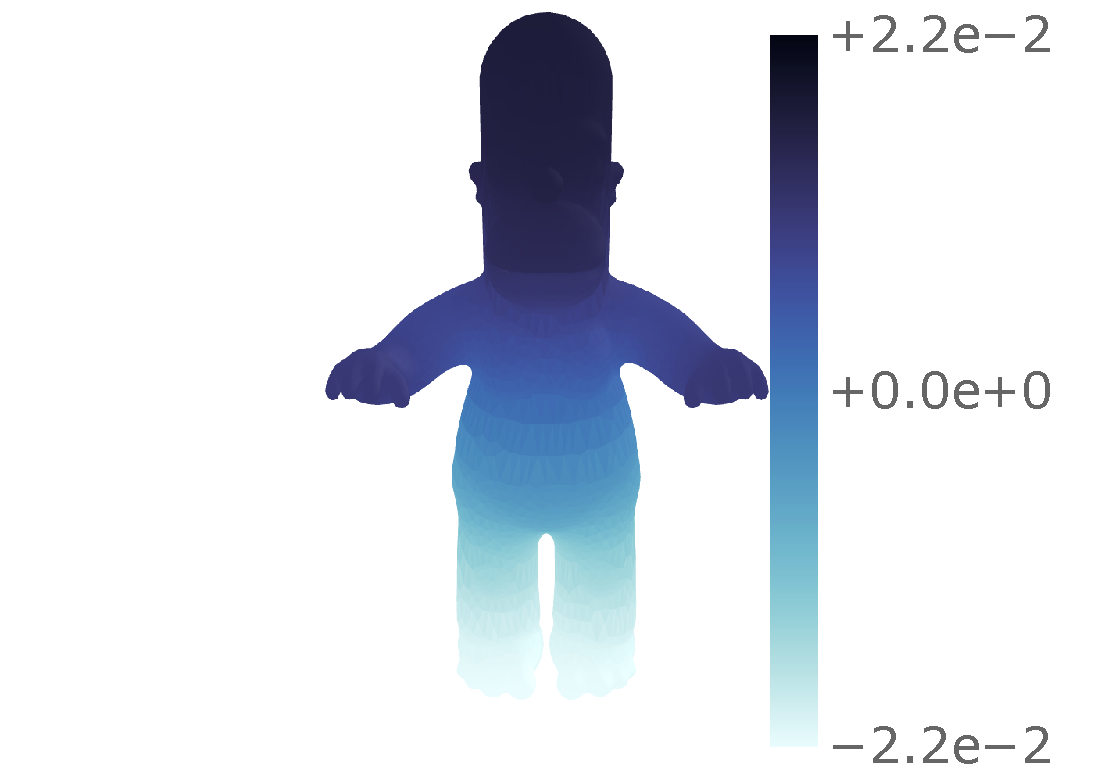
\includegraphics[trim={156 8 21 6},clip,width=.25\textwidth]{homer_rank2_lam1-325328e-03.pdf}} % chktex 8
	\hfill
	\subfloat[\(\mesh{\zeta_{4}}\)]
	{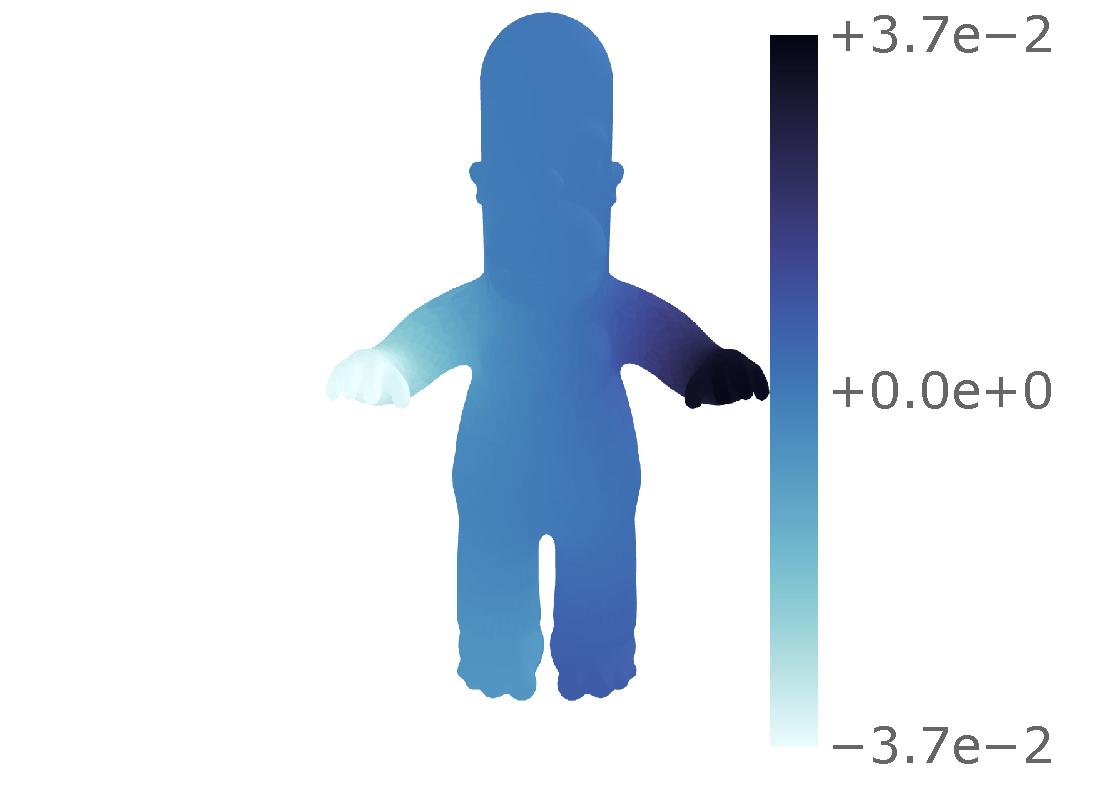
\includegraphics[trim={156 8 21 6},clip,width=.25\textwidth]{homer_rank3_lam2-425344e-03.pdf}} % chktex 8
	\hfill
	\subfloat[\(\mesh{\zeta_{5}}\)]
	{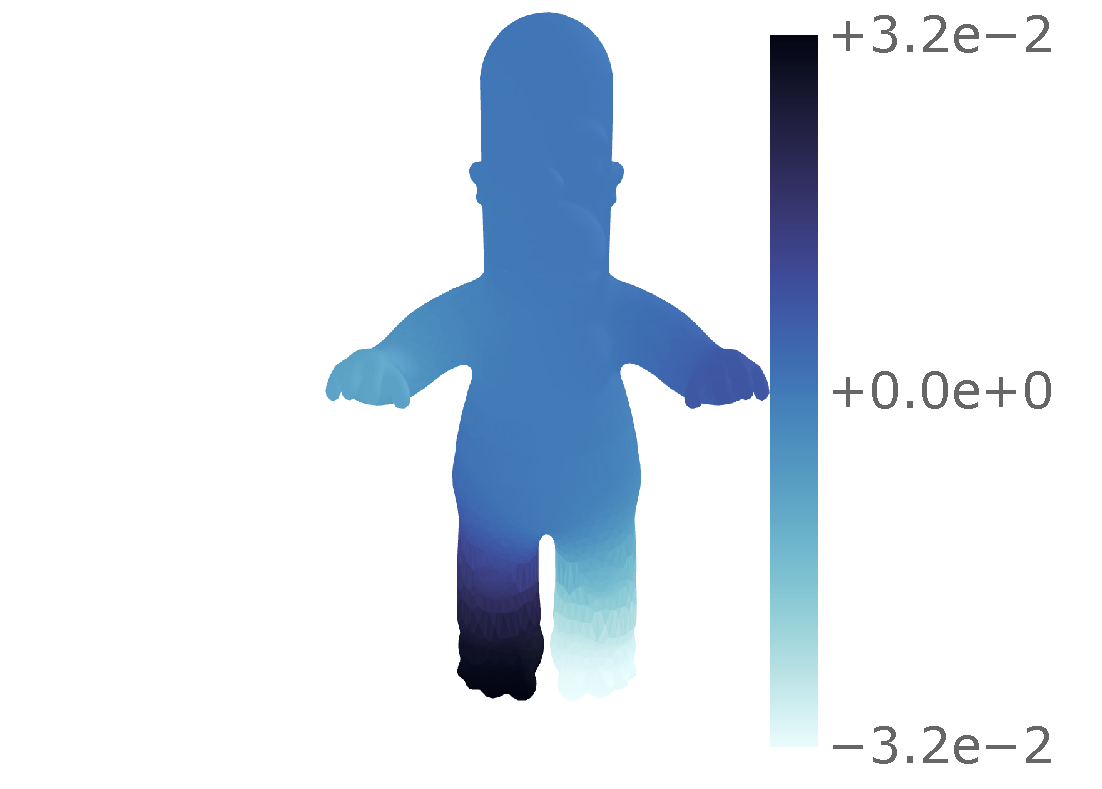
\includegraphics[trim={156 8 21 6},clip,width=.25\textwidth]{homer_rank4_lam2-706937e-03.pdf}} % chktex 8
	\hfill
	\subfloat[\(\mesh{\zeta_{6}}\)]
	{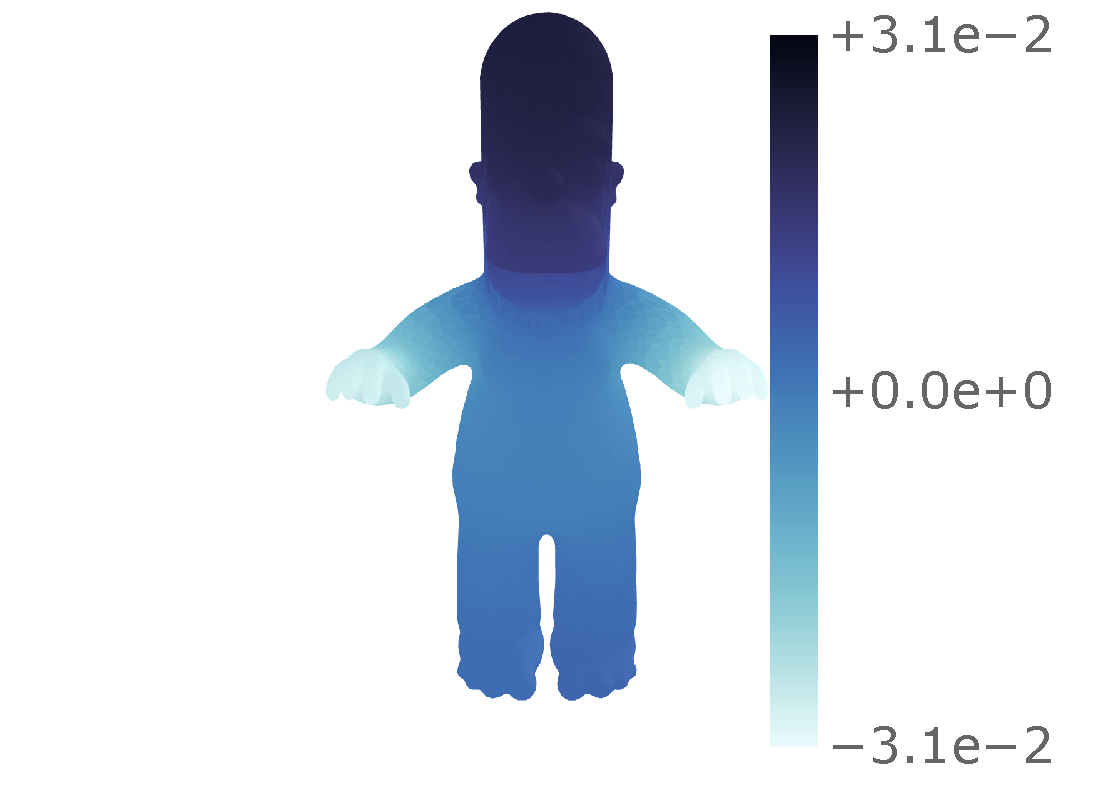
\includegraphics[trim={156 8 21 6},clip,width=.25\textwidth]{homer_rank5_lam2-851096e-03.pdf}} % chktex 8
	\newline
	\subfloat[\(\mesh{\zeta_{7}}\)]
	{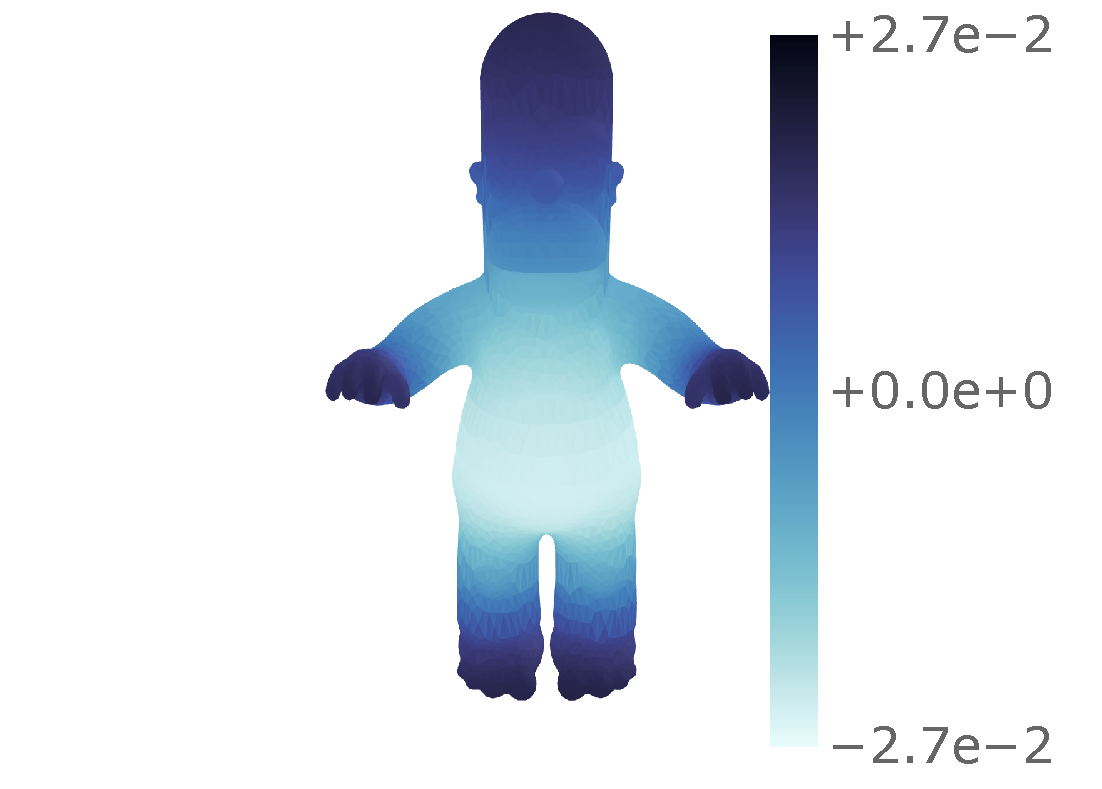
\includegraphics[trim={156 8 21 6},clip,width=.25\textwidth]{homer_rank6_lam7-806422e-03.pdf}} % chktex 8
	\hfill
	\subfloat[\(\mesh{\zeta_{8}}\)]
	{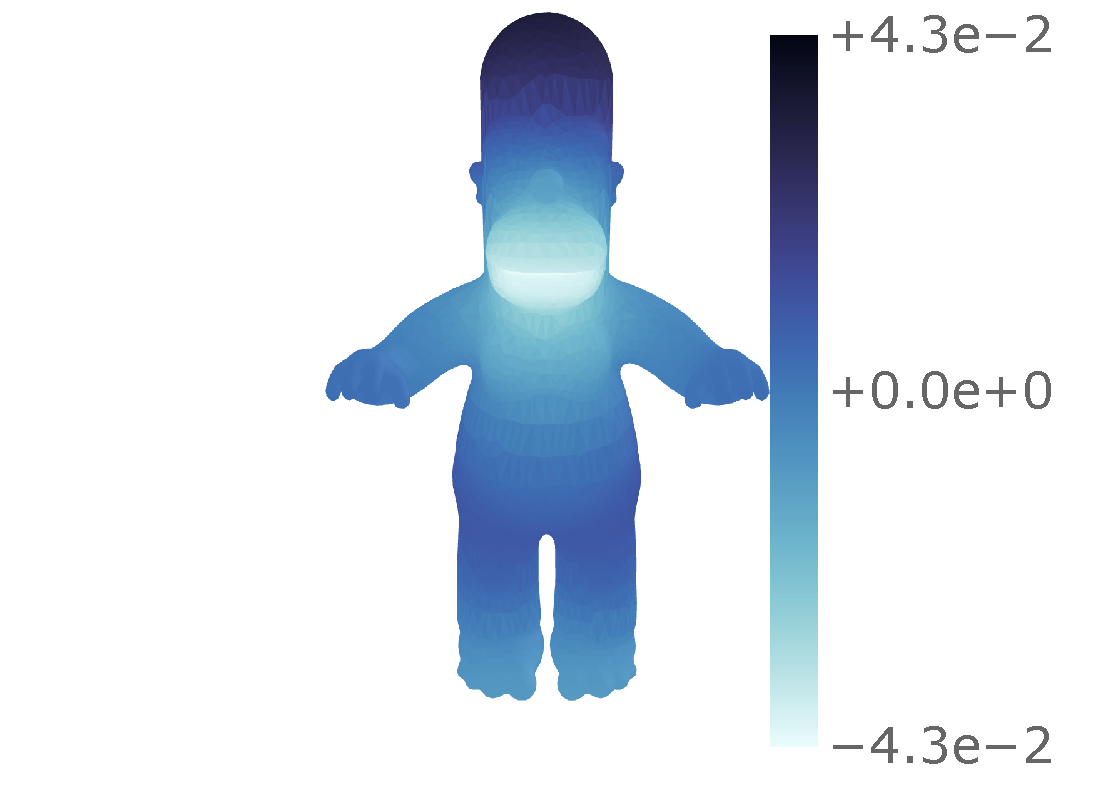
\includegraphics[trim={156 8 21 6},clip,width=.25\textwidth]{homer_rank7_lam1-164387e-02.pdf}} % chktex 8
	\subfloat[\(\mesh{\zeta_{9}}\)]
	{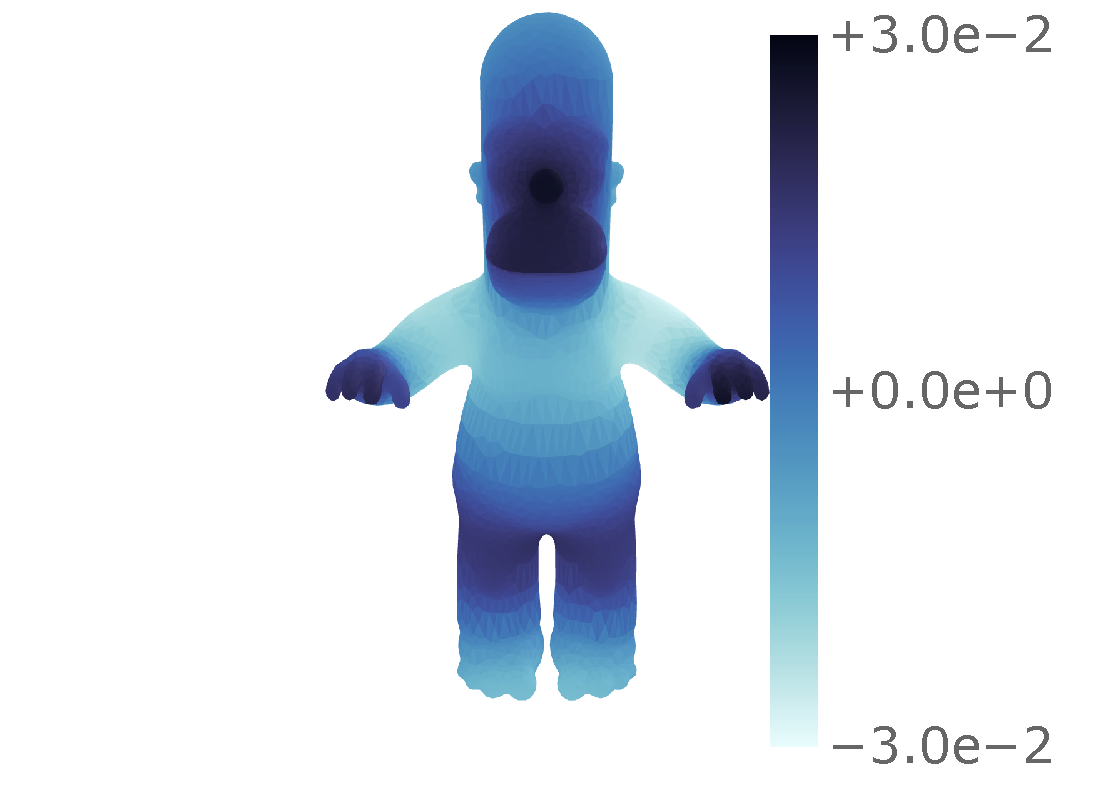
\includegraphics[trim={156 8 21 6},clip,width=.25\textwidth]{homer_rank8_lam1-738974e-02.pdf}} % chktex 8
	\hfill
	\subfloat[\(\mesh{\zeta_{10}}\)]
	{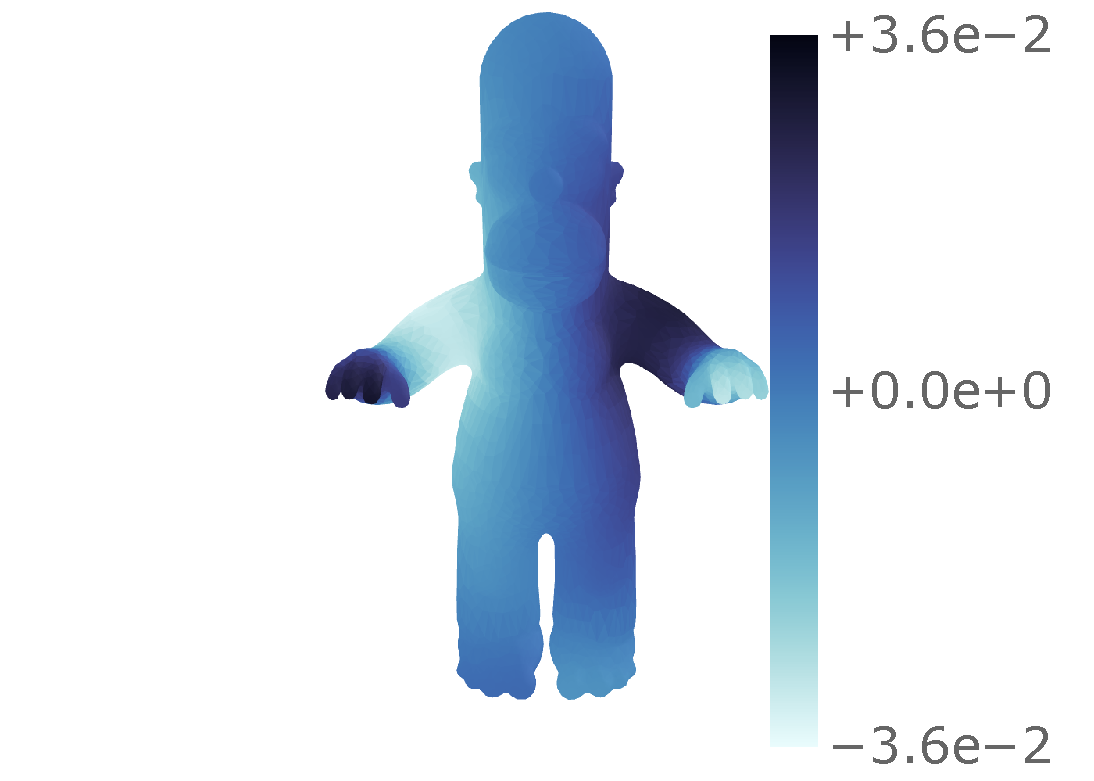
\includegraphics[trim={156 8 21 6},clip,width=.25\textwidth]{homer_rank9_lam1-827015e-02.pdf}} % chktex 8
	\caption[
		Some eigenvectors of the mesh Laplacian of an example mesh
	]{
		The third to tenth eigenvectors of the mesh Laplacian of a Homer Simpson mesh ordered by increasing eigenvalue (frequency).
		In total \(\imax=\num{1275}\) basis functions of the \(\num{5103}\) vertex mesh were computed.
		Whilst the eigenvectors are defined on the vertices, the values have been averaged onto the faces for the plot.
	}\label{fig:chapter5_eigenhomers}
\end{figure}
